\documentclass[utf8]{article}
\usepackage{caption}
\usepackage{graphicx, subfig}
\usepackage{amsmath}
\usepackage{amsfonts}
\usepackage{amssymb}
\usepackage{geometry}
\usepackage{enumerate} 
\usepackage{graphicx}
\usepackage{indentfirst}
\usepackage{subcaption}
\usepackage{multirow}
\usepackage{float}
\usepackage{url}
\linespread{1.5}
\begin{document}
\begin{center}
\vspace*{2cm}
\rule{14cm}{0.5pt}\\
\Large{\textsc{UM-SJTU Joint Institute\\
Intro to Signals and Systems\\
(VE216)\\}}
\rule{14cm}{0.5pt}\\
\vspace*{3cm}
\Large{\textsc{Laboratory Report\\
Lab 1\\
LTI System}}
\vspace*{3cm}
\end{center}
\large{Name: Yiyang Xu\qquad ID:518370910020\\
Date: 9 June 2020}
\newpage

\section{Objectives}
{
	In this laboratory I will construct and test my own uperherodyne AM receiver, which operates on the basis of the same principles used in any radio in my car or home. I will use my radio to listen to both a local commercial AM station broadcast at a carrier frequency of 1600 KHz and to an AM signal transmitted in the laboratory. I will also measure the response of my circuit, at a variety of test points, to a simple AM signal produced by a function generator. The goals of this lab are:
\begin{itemize}
\item Learning resonance phenomena and simple RLC bandpass filters.
\item Learning a bit about antennas.
\item Learning basic superheterodyne receiver operating principles, since theses principles play a critical role in many radio and signal processing systems.
\item Using the frequency domain concepts learned in VE 216 lectures to analyze the operation of a
superheterodyne AM radio receiver. Learn about mixing and its effect on the signal spectrum. Observe the demodulation of an AM signal using an envelope detector.
\item Constructing a fully operational superheterodyne AM radio and demonstrate that it operates as predicted by theory.
\item Gaining an appreciation of the fact that the mathematical tools I have learned in VE 216 can be used to design and build interesting and useful systems.
\end{itemize}
}

\section{Background Information}
Fundamentally, AM modulation and demodulation are based on the Fourier transform modulation property, $$ s(t)\cos(\omega_{LO}t)\leftrightarrow \frac{1}{2}S(j(\omega-\omega_{LO}))+\frac{1}{2}S(j(\omega+\omega_{LO})) $$
The actual translation of this mathematical fact into a practical electrical system of a functioning radio is discussed here. The development is rather long and covers the design of a radio from the antenna all the way to the last stage of demodulation.

In Figure 1, we will find a block diagram of the superheterodyne AM radio that we will be building and testing in this lab.

\begin{figure}[H]
	\begin{small}
		\begin{center}
			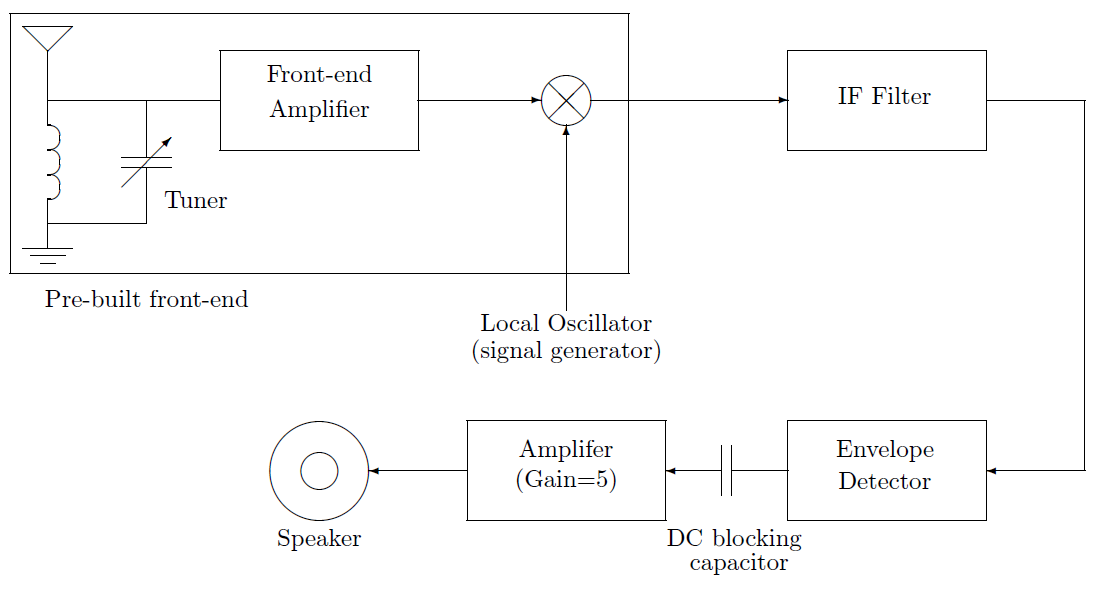
\includegraphics[width=0.75\textwidth]{figures/Figure1.png}
		\end{center}
		\caption{AM Superheterodyne Radio Block Diagram}
		\label{fig:fig1}
	\end{small}
\end{figure}


\subsection{Transmitted Signal}
{
	The transmitted AM (amplitude modulated) signal is of the form $x(t) = ( A + bs(t))\cos(\omega_ct + \phi)$. In Lab 2, we observed signals $x(t)$ of this form with $s(t)$ a sinusoid or a triangular wave. The carrier is specified by $\cos(\omega_ct + \phi)$, $f_c = \omega_c/2\pi$ is the carrier frequency in $Hz$, $s(t)$ is the “information or message” that is being sent, $e.g.$, voice, data, or music, and $A$ and $b$ are constants. The constants $A$ and $b$ are chosen to ensure the condition $A + bs(t) \ge 0$, which, from Lab 2, we know to be important for envelope detection. The modulation depth, specified as a percentage, is defined as
$$\frac{\max(bs(t))-\min(bs(t))}{2A}\times 100\%$$
in Lab 2.
In commercial broadcast AM, the US Federal Communications Commission (FCC) specifies that the carrier frequency must be one of the following 117 values
$$f_c = 540 KHz + (i-1)\times 10 KHz, \quad i = 1, 2, \cdots, 117$$
and thus spans a range from 540 KHz to 1700 KHz in increments of 10 KHz. The carrier frequencies given by this formula correspond to the frequencies on your radio dial (AM).
The information signal itself, $s(t)$, is a baseband signal with a bandwidth of 5 KHz, $i.e.$, $| S(j\omega) | \approx 0$ for $\omega > 2\pi \cdot 5000 rad/s$, where $S(j\omega)$ is the Fourier transform of a long segment of the signal (music, data or voice), $s(t)$. Thus the information signal contains little power at frequencies beyond 5 KHz. Younger adults can hear frequencies up to nearly 20 KHz, and thus commercial AM broadcasts do not transmit music with high fidelity, even in the absence of noise. This is not a limitation imposed by the method of amplitude modulation per se, but rather a consequence of the narrow bandwidth assigned by the FCC when broadcast AM radio was created. We could change this at any time if we were willing to absorb the huge cost of replacing the thousands of transmitters and millions of receivers in existence today.
}

\subsection{Pre-built Front-end: Antenna and Tuned RLC Circuit}
{
	The “front-end” of the radio you will use in the lab has been pre-built and packaged for you. It consists of a tuned RLC circuit, a field effect transistor (FET) pre-amplifier and a mixer. The tuned RLC circuit, in addition to providing some filtering, also serves as an antenna. The antenna/tuned RLC circuit can be modeled by the circuit shown in Figure 2 below.

	\begin{figure}[H]
		\begin{small}
			\begin{center}
				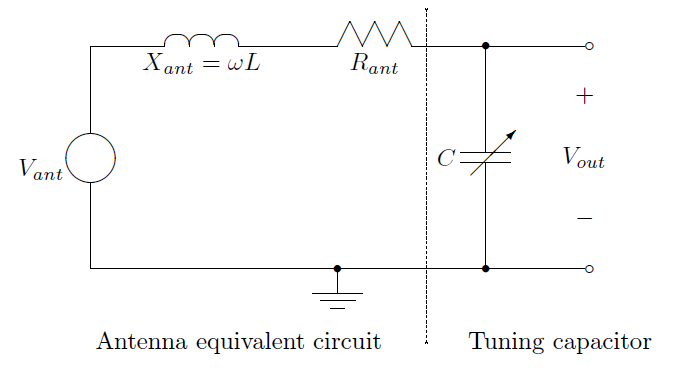
\includegraphics[width=0.75\textwidth]{figures/Figure2.png}
			\end{center}
			\caption{Antenna/Front-end Tuned RLC Circuit (preamplifier and mixer not shown)}
			\label{fig:prebuilt}
		\end{small}
	\end{figure}

	As will be described later, the inductor value is fixed at approximately 960 $\mu H$, the antenna resistance $R_{ant}$ is frequency dependent, increasing with frequency, and $C$ is a user-controllable variable capacitor. It is a straightforward exercise to compute $V_{out}(j\omega)/V_{ant}(j\omega)$ as a function of frequency $\omega$. It will be assumed that the output of the circuit is connected to a very high impedance input (e.g., the input of a field effect transistor (FET)), and thus is essentially open-circuited. The quantity $20\log|V_{out}(j\omega)/V_{ant}(j\omega)|$  dB has been computed and is plotted in Figure 3 for two different RLC combinations which are antenna and tuning,

	\begin{figure}[H]
		\begin{small}
			\begin{center}
				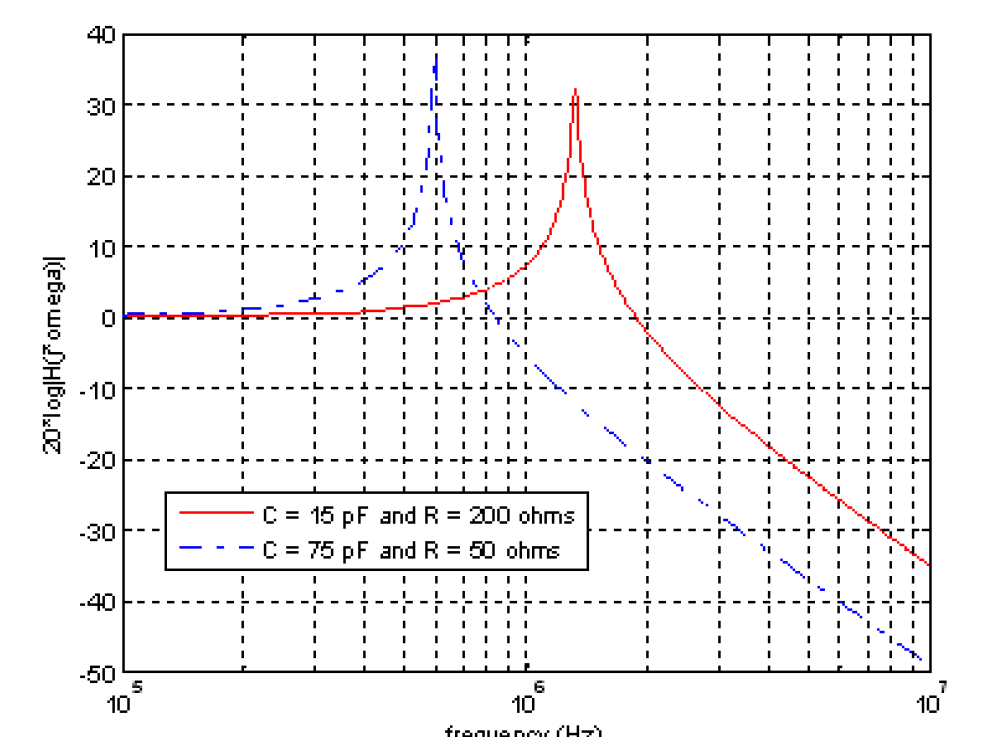
\includegraphics[width=0.75\textwidth]{figures/Figure3.png}
			\end{center}
			\caption{}
			\label{fig:front-end}
		\end{small}
	\end{figure}

	i.e., $R_{ant} = 200 \Omega$, $L = 960 \mu H$, $C = 15 pF$ and $R_{ant} = 50 \Omega$, $L = 960 \mu H$, $C = 75 pF$. Note that this circuit acts as a bandpass filter whose center frequency is determined by the value of the capacitor, which is tunable by the radio listener. The capacitor value is chosen by the listener so that the center frequency of the bandpass filter corresponds to the carrier frequency of the desired AM station.
}

\subsubsection{Antenna (or How to Efficiently Receive a Signal)}
{
	An antenna is a device that provides a means of transmitting or receiving radio waves, i.e., electromagnetic signals that propagate through free-space. Antennas are common components of almost every communication device, from radios to cellphones to laptops.
	Antennas can take many different forms depending on the application. In our radio, the receiving

	antenna is a coil of wire wound around a ferrite core, $i.e.$, an electrically non-conducting material with special magnetic properties. Such a coil depicted in Fig. 4(a) is known as a “loopstick” and is commonly used for the antenna in AM radios.

	\begin{figure}[H]
		\begin{small}
			\begin{center}
				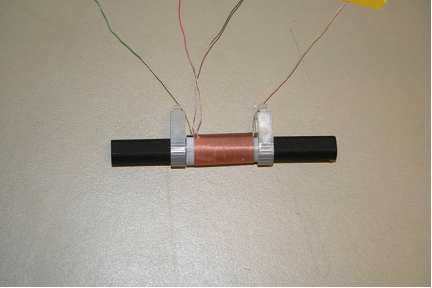
\includegraphics[width=0.75\textwidth]{figures/Figure4.png}
			\end{center}
			\caption{(a) A Loopstick Antenna}
			\label{fig:antenna}
		\end{small}
	\end{figure}

	The carrier wavelength, $\lambda_c$, is given by $\lambda_c = c/f_c$, where $c$ is the vacuum speed of light, $3\times10^8 m/s$, and $f_c$ is the carrier frequency in Hz, which for commercial AM lies between 540 KHz and 1700 KHz. Thus the carrier wavelength is on the order of a few hundred meters. The electrical properties of an antenna can be modeled by a Thevenin equivalent circuit consisting of a voltage source, $V_{ant}$, in series with an impedance, $Z_{ant} = R_{ant} + jX_{ant}$ as shown in Figure 6.

	\begin{figure}[H]
		\begin{small}
			\begin{center}
				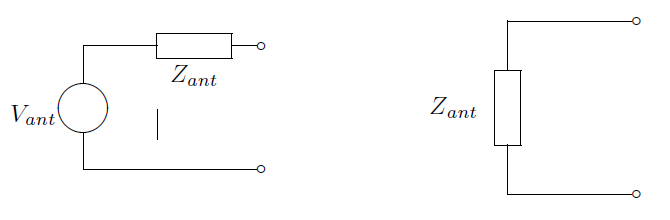
\includegraphics[width=0.75\textwidth]{figures/Figure6.png}
			\end{center}
			\caption{Thevenin Equivalent Circuit Model for an Antenna (a) Receiving, (b) Transmitting}
			\label{fig:thevenin}
		\end{small}
	\end{figure}
	

	$Z_{ant}$ is the same whether the antenna is transmitting or receiving a signal. $V_{ant}$, on the other hand, is only non-zero when the antenna is receiving a signal. Time-varying electric and magnetic fields are associated with the transmission of radio waves. According to Faraday’s Law of electromagnetic, a time-varying magnetic field radiated from a distant transmitter will induce an (open-loop) voltage drop, $V_ant$, across the ends of the coil in a loopstick receiving antenna (in particular, the voltage induced across the ends of a loop of wire equals the rate of change of flux through that loop). The voltage drop will be proportional to the product of the square-root of the power of the transmitted radio wave measured at the receiving antenna, the cross-sectional area of the coil, the number of turns in the coil and the relative permeability of the ferrite core.

	$R_{ant}$ is the sum of three resistive terms (1) the radiation resistance $R_r$ of the antenna, (2) the resistance $R_{coil}$ of the coil wire and (3) the magnetic losses (due to hysteresis) in the core $R_{core}$,
	$$R_{ant} = R_r + R_{coil} + R_{core}$$
	The coil wire and the core magnetic losses are parasitic effects, and with ideal materials ($i.e.$, perfectly conducting coil wires and ferrites without hysteresis), these resistive terms would be zero. The radiation resistance, as the name implies, is associated with the radiation and reception of electromagnetic radiation ($i.e.$, radio waves) and is not actually a loss term. If a sinusoidal voltage source is applied across the ends of the antenna coil when used as a transmitting antenna, a current will flow in the coil. The ratio of the applied voltage to current, assuming that $R_{coil}$ and $R_{core}$ are zero, is given by the radiation resistance. Furthermore the time-averaged power radiated away from the antenna in the form of an electromagnetic wave is given by the product of 1/2 the square of the current and the radiation resistance ($i.e.$, the power that would be dissipated by a real resistor of $R_{ant}$ ohms). Similarly when operated as a receiving antenna, the current flowing through an attached load of impedance $Z_L$ will be given by $I_L = V_{ant}/(Z_{ant} +Z_L )$. This current not only delivers signal power to the load but also drives the antenna to re-radiate some of the received electromagnetic signal. The time-averaged power that is re-radiated is given by the product of 1/2 the square of the current and the radiation resistance.

	The radiation resistance of a loopstick receiving antenna is negligible ($\ll$ 1 ohm) when the size of the antenna is small relative to a wavelength (as it is in our case) and can be ignored. The coil and ferrite core resistance values increase with frequency, but together remain below a few hundred ohms at commercial AM carrier frequencies. The reactance of the antenna is inductive and corresponds to an inductor value of approximately 960 $\mu H$ for our loopstick. The use of a ferrite core, as opposed to a hollow air core, greatly increases (by a factor of several hundred to a thousand) the strength of the magnetic field inside the coil, and hence the Thevenin equivalent voltage, $V_{ant}$. It also increases the inductance by an identical multiplicative factor.

	In general, why should one care about the impedance of an antenna? Well suppose that the antenna is being used for transmission. The output of the transmitter, which generates some voltage, is applied across the antenna terminals. The transmitter output can be modeled as Thevenin equivalent voltage, $V_{trans}$, in series with a Thevenin equivalent impedance, $Z_{trans}$. The power radiated by the antenna will then be given by
	$$ P_{rad} = \frac{1}{2}\mid\frac{V_{trans}}{Z_{ant}+Z_{trans}}\mid^2 R_{ant} $$
	This power will be a maximum when the transmitter is designed to yield $R_{trans} \approx 0$ and $X_{trans} = - X_{ant}$, yielding
	$$ max(P_{rad}) = \frac{1}{2}|\frac{V_{trans}}{R_r+R_{core}+R_{coil}}|^2R_r^2$$
	Thus the fraction of the power radiated by the antenna (as opposed to being dissipated “needlessly” in the coil and core) is given by
	$$(\frac{R_r}{R_r+R_{core}+R_{coil}})^2$$
	Clearly the efficiency increases as the size of $R_{coil} + R_{core}$ can be reduced relative to the radiation resistance. Unfortunately, antennas that are small relative to the wavelength of the signal being transmitted generally have very small radiation resistances and thus are inefficient radiators.

	A similar analysis can be performed when the antenna is used for reception rather than transmission.

	The received power dissipated in $R_{coil} + R_{core}$ is wasted. Furthermore, the issue of noise becomes important. The ability to communicate with high fidelity is ultimately limited by the presence of noise$/$interference. Some noise is present in the atmosphere, for example that due to lightning strikes around the world, while some is produced by the electronics themselves inside the radio. It is a fundamental fact of physics that it is impossible to completely remove the electronics noise because it is due to the thermal agitation of electrons in the circuit elements. In situations where the external atmospheric noise is negligible in comparison to the signal level and the signal level is very weak, it is important to deliver as much of the received signal as possible to the load in order to overcome the noise due to the radio electronics. We know that maximum power delivery from the antenna to the load occurs when the impedance of the load is matched to that of the antenna. Let us assume for the moment that we have an antenna with very low parasitic resistance, $R_{coil} + R_{core}$, which is good from an efficiency point of view. In order to deliver maximum power from the antenna to the load under such conditions, the front-end receiver electronics must be designed to be impedance matched, $i.e.$, $Z_{load} = Z_{ant}^{*}$ . For small (relative to the wavelength) antennas, however, this is very difficult to achieve because $R_r$ is very small.

	In the AM radio band, atmospheric noise and interference are generally much larger than the electronics noise. Thus the fidelity is not limited by the electronics noise and therefore impedance matching of the load to the antenna is not critical as long as a reasonable signal level is provided to the load.
}

\subsubsection{RLC Resonant Circuit (or the First Step in Selecting a Station)}
{
	The variable capacitor indicated in Figure  consists of two sets of interleaved parallel metallic plates as shown in Figure 5(b). One set of the plates can be rotated relative to the other, thus varying the overlap between the two plate sets, which in turn causes the capacitance to change. The capacitance ranges from about 10 pF when there is no overlap between the plates to 400 pF when the plates are fully overlapped.

	\begin{figure}[H]
		\begin{small}
			\begin{center}
				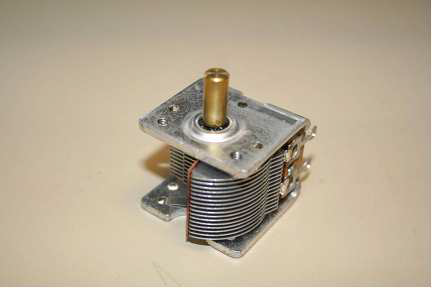
\includegraphics[width=0.75\textwidth]{figures/Figure5.png}
			\end{center}
			\caption{(b) Variable Capacitor}
			\label{fig:antenna_2}
		\end{small}
	\end{figure}

	The loopstick antenna together with the capacitor shown in Figure is a series RLC resonance circuit. Since this type of circuit and resonance phenomena in general play such an important role in electrical engineering, we will digress briefly to discuss these topics in some further detail below.

	The current flowing in the RLC circuit will be a maximum when the series RLC impedance is minimum. This impedance minimum occurs at a frequency for which the reactance of the inductor ($i.e.$, $j\omega L$) exactly cancels the reactance of the capacitor ($i.e.$, $−j/\omega C$). When this condition occurs, the circuit is said to be at resonance. The resonance frequency is given by
	$$f_{res} = \frac{1}{2\pi}\frac{1}{\sqrt{LC}}Hz \quad or \quad \omega_{res} = \frac{1}{\sqrt{LC}}$$
	and at the resonance frequency, the current achieves its peak value of $V_{ant}/R_{ant}$. The magnitude of the current decreases monotonically as one moves away from resonance. The current drops to $1/\sqrt{2}$ of its peak value when the source frequency is given by
	$$ f = \frac{1}{2\pi}\sqrt{\frac{1}{LC}+(\frac{R}{2L})^2} \pm \frac{1}{2\pi}\frac{R}{2L} Hz$$
	Thus the 3 dB bandwidth, $BW_{3dB}$, of the resonant response is equal to
	$$BW_{3dB} = \frac{1}{2\pi}\frac{R}{L}Hz$$
	While the resonance frequency does not lie exactly at the midpoint between the two 3 dB points, it is very nearly centered when $BW_{3dB}\ll f_{res}$.
	The ratio $f_{res}/BW_{3dB}$ measures the “sharpness” of the resonance and is known as the quality factor, or $Q$ of the circuit. Using equations above, it is easily shown that
	$$Q = 2\pi f_{res}\frac{L}{R}$$

	A high $Q$ corresponds to a very sharp resonance, $i.e$, $BW_{3dB}\ll f_{res}$. Note that the $Q$ is inversely proportional to $R$, which is the source of power dissipation in the resonator. Consequently $Q$ increases as the resonator losses decrease. The combination of the loopstick antenna and variable capacitor act as a tunable bandpass filter as we saw in Figure 3. Placing the resonance peak at the carrier frequency of the desired radio station is the first step in receiving a signal and rejecting unwanted signals.

	Continuing with our discussion of the radio front-end, the inductance of the loopstick antenna has been measured to be approximately 960 $\mu H$ while the variable capacitor has a range of about 10 pF to 400 pF. The bandwidth of the front-end resonant circuit is given by $BW_{3dB} = \frac{1}{2\pi}\frac{R}{L}Hz$. Thus in order to estimate the bandwidth, we need to know the value of $R_{ant}$, which as we indicated earlier is determined primarily by the loopstick coil resistance and the losses in the ferrite core. By replacing the voltage source, $V_{ant}$, shown in Figure 2 by a function generator and measuring the resonant 3 dB bandwidth for different capacitance values, one can determine $R_{ant}$ as a function of the resonance frequency. As noted earlier, the value of $R_{ant}$ will increase with frequency, and thus the $Q$ of the filter will decrease, $i.e.$, the filter will become less frequency selective, as the resonance frequency increases.

	We have also seen in lecture that the time-domain and frequency-domain descriptions of LTI systems are related via the Fourier transform. Namely the time response of an LTI system is given by the convolution of the input with the system’s impulse response, and the frequency response is the product of the Fourier transform of the input and the frequency response function. In addition, the frequency response function is equal to the Fourier transform of the impulse response. Finally, the impulse response is equal to the derivative of the step response.

	If we consider the series RLC circuit shown in Figure 2, it is easy to verify that $V_{ant}$ and $V_{out}$ are related by the following differential equation by noting that the sum of the voltage drops around the loop must be zero
	$$LC\frac{d^2V_{out}}{dt^2}+RC\frac{dV_{out}}{dt}+V_{out} = V_{ant}$$
	If we set the $V_{ant}$ to be a unit step function, then the solution to the equation is given by
	$$V_{out} = [1-(\sin\phi)^{-1}e^{-(R/2L)t}\sin(\omega t+\phi)]u(t)$$
	where
	$$\omega = \sqrt{\omega_{res}^2-(R/2L)^2}rad/s$$
	$$\phi = \tan^{-1}(\frac{\sqrt{\omega_{res}^2-(R/2L)^2}}{(-R/2L)})$$
	$$\omega_{res} = \frac{1}{\sqrt{LC}}rad/s$$
	Observe that the step response has an exponentially decaying sinusoidal component. When the $Q$ is high, the oscillating frequency will be approximately equal to the resonance frequency, $\omega_{res}$, while the resonant bandwidth is related to the exponential decay rate, $R/2L$. These observations can be used to determine the resonance frequency and the bandwidth experimentally.
}


\subsection{First Stage of Demodulation: The Amplifier and Mixer in the Front-end}
{
	The output of the circuit shown in Figure 2 is fed into a single field-effect transistor (FET) amplifier to boost the signal strength to a level suitable for the mixer to operate. The output of this amplifier feeds one of the two mixer inputs. The mixer is a nonlinear device that produces at its output the product of the voltages appearing at its two input ports (designated signal port and LO port). The local oscillator (LO) input is a sinusoid whose frequency is varied to select the channel ($i.e.$, 540 KHz through 1700 KHz) to which one wishes to listen. For our radio, the LO is the signal generator on your lab bench. Thus for a transmitted AM signal
	$$x(t) = (A + bs(t))\cos(\omega_c t+\phi)$$
	the output of the mixer will be given by
	$$(A+bs(t))\cos(\omega_c t+\phi)\cos(\omega_{LO} t + \theta)$$
	where $\theta - \phi$ is the relative phase difference between the carrier and the LO. The receiver has no way of knowing the value of this phase difference. A little bit of trigonometry ($i.e.$, $\cos(x) \cos(y) = \frac{1}{2} \cos(x + y)+ \frac{1}{2} \cos(x − y))$ indicates that
	$$(A+bs(t))\cos(\omega_ct+\phi)\cos(\omega_{LO}t+\theta) = \frac{1}{2}(A+bs(t))\cos((\omega_c+\omega_{LO})t+\phi+\theta)+\frac{1}{2}(A+bs(t))\cos((\omega_c-\omega_{LO})t+\phi-\theta)$$
	Note that mixing has both translated the carrier frequency of the original signal up to a frequency of $\omega_c+\omega_{LO}$ and down to a frequency $\omega_c-\omega_{LO}$, as guaranteed by the following Fourier transform property: $x(t)\leftrightarrow X(j\omega)$ implies that
	$$x(t)\cos(\omega_0t)\leftrightarrow\frac{1}{2}X(j(\omega+\omega_0))+\frac{1}{2}X(j(\omega-\omega_0))$$
	A frequency domain representation of the operation of the modulator and mixer is illustrated in Figure 7

	\begin{figure}[H]
		\begin{small}
			\begin{center}
				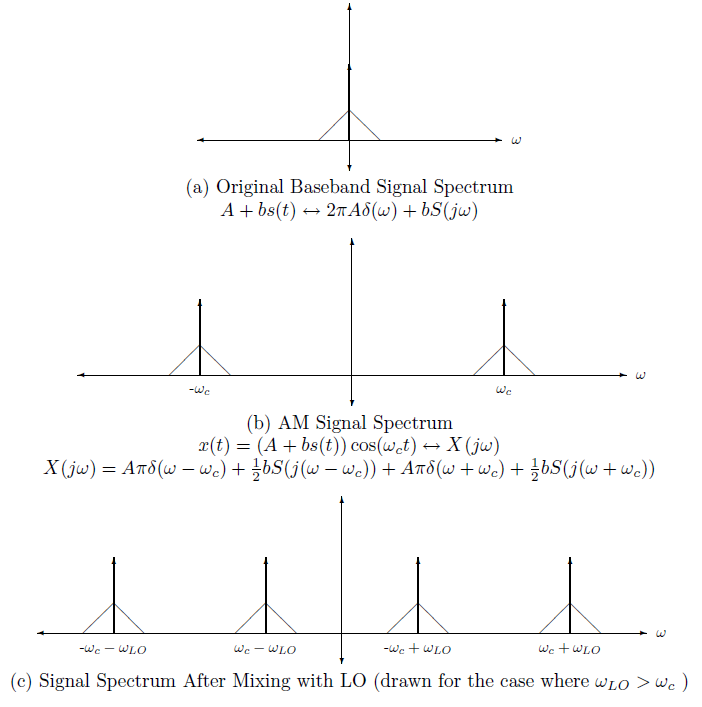
\includegraphics[width=0.65\textwidth]{figures/Figure7.png}
			\end{center}
			\caption{Signal Spectrum (a) original signal, (b) signal at transmitter after AM modulation, (c) signal at the output of the radio front-end mixer.}
			\label{fig:spectrum}
		\end{small}
	\end{figure}
	
	For simplicity of illustration,we have assumed that the spectrum of $s(t)$ is purely real, has a triangular shape, and that $\theta = \phi = 0$.
}

\subsection{IF Filter or How to Practically Select a Station and Demodulate a Signal}
{
	The intermediate frequency (IF) filter shown in Figure 1 is a bandpass filter centered at fIF (the IF frequency). In the ideal case, the frequency response function of this filter would be that shown in Figure 7 below. Observe (see Figure 7 (c)) that by choosing the LO frequency appropriately we can use the mixer

	\begin{figure}[H]
		\begin{small}
			\begin{center}
				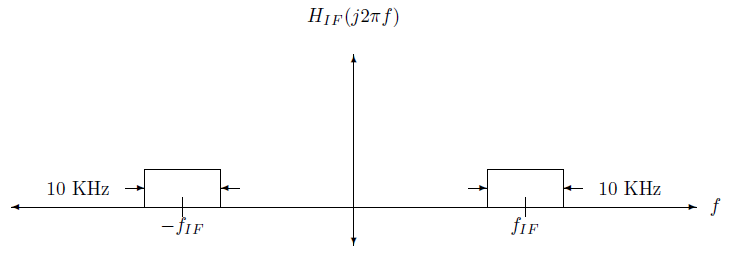
\includegraphics[width=0.75\textwidth]{figures/Figure8.png}
			\end{center}
			\caption{Ideal IF Filter}
			\label{fig:idealif}
		\end{small}
	\end{figure}

	to shift the frequency of the modulated signal so that the modulated signal passes through the IF filter undistorted (assuming, of course, that the bandwidth of the IF filter exceeds the bandwidth of the message signal). Either of two frequency choices are possible for the LO, namely (assuming $f_c > f_{IF}$)
	$$\omega_{IF} = \omega_c-\omega_{LO}\rightarrow f_{LO} = f_c-f_{IF}$$
	or
	$$\omega_{IF} = -\omega_c+\omega_{LO}\rightarrow f_{LO} = f_c+f_{IF}$$
	as indicated below in Figure 9 and 10, respectively.

	\begin{figure}[H]
		\begin{small}
			\begin{center}
				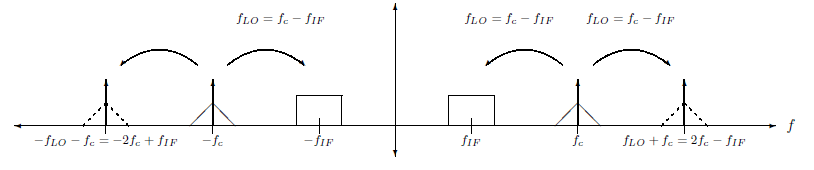
\includegraphics[width=0.75\textwidth]{figures/Figure9.png}
			\end{center}
			\caption{Using LO to Mix into IF Band when $f_{LO} = f_c − f_{IF}$}
			\label{fig:LO-IF-}
		\end{small}
	\end{figure}
	\begin{figure}[H]
		\begin{small}
			\begin{center}
				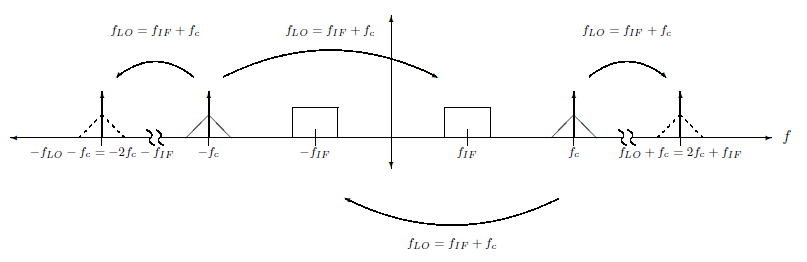
\includegraphics[width=0.75\textwidth]{figures/Figure10.png}
			\end{center}
			\caption{Using LO to Mix into IF Band when $f_{LO} = f_{IF} + f_c$}
			\label{fig:LO-IF+}
		\end{small}
	\end{figure}
	
	In either case the output of the IF filter (up to a multiplicative constant) becomes
	$$(A+bs(t))\cos(\omega_{IF}t+\phi-\theta)$$
	Thus, if the output of the IF filter is fed into a properly designed envelope detector (see Lab 2), the output of the envelope detector will be $A + bs(t)$ (up to a multiplicative constant). Finally the constant term, $A$, can be removed by placing a capacitor in series with the output of the envelope detector (see Figure 1) to block the DC component, leaving just the information signal $s(t)$ (up to a multiplicative constant). Thus our radio will have recovered the transmitted information signal, $s(t)$! A similar result is obtained when $f_c < f_{IF}$.
}


\subsection{A Simple Butterworth Filter Realization of the IF Filter}
{
	We have seen that the IF filter should be a bandpass filter. Bandpass filters can take many different forms. For example, a bandpass Butterworth filter of order N is characterized by the following (magnitude) frequency response function
	$$|H(j\omega)|^2 = \frac{H_0}{1+[2(\omega-\omega_0)/\beta]^{2N}}$$
	where the center frequency of the filter is $\omega_0 rad/s$, the peak gain is $H_0$ and the 3-dB bandwidth is $\beta rad/s$. This filter approaches an ideal bandpass filter as $N$ gets large, since for $N$ large, the frequency response function is nearly constant and equal to $H_0$ over the passband, $|\omega − \omega_0| < \beta$, and decreases rapidly towards zero as one moves outside of the passband. Note that the 3-dB bandwidth alone does not indicate the sharpness of the transition from passband to stop band. For the Butterworth filter, both the 3-dB bandwidth and the filter order N determine the filter performance.

	In this lab, we will construct a very simple, op amp-based, IF filter. This filter does not have a particularly sharp passband-to-stopband transition, but it is relatively simple to build and will be sufficient for our application.

	The frequency response function of our bandpass filter is given by
	$$H(s) = H_0\frac{\beta s}{s^2+\beta s+\omega_0^2}$$
	where $s = j\omega$. Note that the equation above can be rewritten as
	$$H(j\omega) = H_0\frac{\beta j \omega_0}{(\omega_0+\omega)(\omega_0-\omega)+j\beta\omega} = H_0\frac{1}{\frac{\omega}{\omega_0}+j\frac{\omega-\omega_0}{\beta\omega_0/(\omega_0+\omega)}}$$

	For $\omega$ in the vicinity of $\omega_0$, the equation reduces to
	$$H(j\omega)\approx H_0\frac{1}{\frac{\omega}{\omega_0}+j\frac{\omega-\omega_0}{\beta\omega_0/(\omega_0+\omega)}} = H_0\frac{1}{1+j\frac{\omega-\omega_0}{\beta/2}}$$
	It follows that the frequency response function achieves a maximum value of $H_0$ at a frequency of $\omega_0 rad/s$ with a 3-dB bandwidth equal to $\beta rad/s$. Moreover, this result applies to our original frequency response function as long as $\beta + \omega_0\approx\omega_0$, that is, when $\beta$ is a small fraction of $\omega_0$, which one typically writes as $\beta\ll\omega_0$.

	The bottom line is that the bandpass filter achieves a maximum value of $H_0$ at a frequency of $\omega_0 rad/s$ with an approximate 3-dB bandwidth of
	$$BW_{3dB}\approx\beta$$
	valid when
	$$\beta\ll\omega_0$$
	\textbf{Image Frequencies:}
	This discussion is carried out for the case that the carrier frequency is greater than the center frequency of the IF filter.

	By examining Figure 10, one can see that when the LO frequency $f_{LO}$ is set equal to $f_c + f_{IF}$, not only does the signal centered at $f_c$ get mixed into the IF band, but so does any signal centered at
	$$f_{imag} = f_{IF} + f_{LO} = f_c + 2f_{IF}$$

	The frequency band centered at $f_{imag}$ is known as the image band. Using the equation above, we conclude that
	$$f_{imag}-f_c = 2f_{IF}$$
	valid when $f_{LO} = f_c + f_{IF}$ and $f_c >f_{IF}$.

	Thus the separation between the carrier frequency of the desired station and the center frequency of the image band (which also ends up in the passband of the IF filter after the mixer) is equal to twice the IF frequency.

	A similar result is obtained when the situation illustrated in Figure 9 is considered. Specifically, when $f_{LO} = f_c − f_{IF}$,
	$$f_{imag} = |f_{IF}-f_{LO}| = |2f_{IF}-f_c|.$$
	Then the separation between the carrier frequency of the desired station and the center frequency of the image band is equal to
	$$f_c -f_{imag} = 2f_{IF},(f_c>2f_{IF}); 2(f_c-f_{IF}),(f_c<2f_{IF})$$
	valid when $f_{LO} = f_c-f_{IF}$ and $f_c>f_{IF}$.
	We conclude that when the LO frequency is chosen to be the higher of the two possible choices, namely $f_c + f_{IF}$, then the IF filter cannot separate two AM stations whose carrier frequencies differ by twice the IF frequency, and according to the deduced equation, the separation between the desired and image stations may be even less when the lower LO frequency is used. In either case, the RLC front-end (recall the antenna and resonance tuning circuit) must sufficiently attenuate signals in the image band when tuned to the carrier frequency of the desired station; otherwise, the image band will corrupt the demodulation of the desired station. Consequently, the higher LO frequency is often chosen in order to simplify the design of the RLC filter in the front-end. AM radios are designed so that both the LO frequency and the resonance frequency of the RLC front-end are set together when a station is selected. The capacitor in the front-end RLC circuit is adjusted so that the resonance frequency of this circuit is equal to the carrier frequency, $f_c$, of the station that is to be received, while the LO frequency is set to one of the two frequencies $|f_c \pm f_{IF} |$.

	The frequency selectivity ($i.e.$, its $Q$) of a bandpass filter is a measure of its ability to attenuate signals that do not lie near the center frequency of its passband, $i.e.$, within a small fraction of the center frequency of the passband. Consequently if the IF frequency is properly chosen, then the front-end RLC circuit does not need to have much frequency selectivity in order to reject the image frequency because $(f_c-f_{imag})/f_c = 2f_{IF}/f_c$ when $f_{LO} = f_c + f_{IF}$. For example, if $f_{IF}= 455 KHz$, which is a common choice in commercial radios, then the desired and image frequencies are separated by 910 KHz and the front-end series RLC filter does not require much frequency selectivity. The IF filter for the radio that you will build in this lab will be centered at approximately 100 KHz.
}





\section{Experimental Procedure}
{
	\subsection{Modulated Sine Wave}
	{
\begin{enumerate}
		\item I set the load of the function generator to be 50 Ohm.
		\item Use function generator to generate a modulated sine wave with baseband frequency 1kHz and modulating frequency 100kHz.The original signal should have 4V Vpp. The carrier (modulating) signal should be sine wave as well. The modulation depth should be 50$\%$ (modulation index 0.5).
		\item Directly connect the generator to the oscilloscope to verify your generated waveform. Store the images with time division $200\mu s$ and $20\mu s$.
		\item In the post-lab report, give the mathematical formula of this waveform.

	\end{enumerate}}
	}
	
}



\subsection{Modulated Triangular Wave}
{
	\begin{itemize}
\item Repeat Part 1, with the only difference that the original signal should have triangular shape.
\end{itemize}
}


\subsection{Envelope Detector}
\begin{itemize}
\item Assemble the circuit using $R = 75 k\Omega$ and $C = 2.2nF$ according to Figure \ref{setup1}.
\item Use the envelope detector to ”demodulate” the two signals in Part 1 and 2. Store your images still at $T = 200\mu s$ and $20\mu s$. In each image, be sure to display both CH1 (as input) and CH2 (as output).
\end{itemize}
\begin{figure}[htbp]
	\centering
	\includegraphics[width=0.7\linewidth]{fig10.png}
	\caption{Circuit setup for envelope detector.}
	\label{setup1}
\end{figure}
\subsection{Amplifier}
\begin{itemize}
\item  Use the function generator to generate a 5kHz sine wave with 500 mV Vpp.
\item Assemble the circuit using $R_1 = 15k\Omega$, $R_2 = 5.6k\Omega$, $R_3 = 82k\Omega$ and $C = 220\mu F$ according to Figure \ref{setup2}. Capture both input and output on the Ocsilloscope. Compare the measured gain of your amplifier with the calculated value. The instruction for the connection of an amplifier is shown in Figure \ref{amp}.
\end{itemize}
\begin{figure}[htbp]
	\centering
	\includegraphics[width=0.7\linewidth]{fig11.png}
	\caption{Circuit setup for amplifier.}
	\label{setup2}
\end{figure}
\begin{figure}[htbp]
	\centering
	\includegraphics[width=0.7\linewidth]{fig12.png}
	\caption{The nodes of an amplifier.}
	\label{amp}
\end{figure}

\section{Results}
\subsection{Modulated Sine Wave}
\begin{itemize}
\item Time division $200\mu s$ 
\begin{figure}[htbp]
	\centering
		\includegraphics[width=0.7\linewidth]{11.png}
	\caption{The image of modulated sine wave with time division $200\mu s$}
	\label{fig-1-1}
\end{figure}

\item Time division $20\mu s$ 
\begin{figure}[htbp]
	\centering
		\includegraphics[width=0.7\linewidth]{12.png}
	\caption{The image of modulated sine wave with time division $20\mu s$}
	\label{fig-1-2}
\end{figure}
\end{itemize}

\subsection{Modulated Triangular Wave}
\begin{itemize}
\item The original signal should have triangular shape.
\item Time division $200\mu s$ 
\begin{figure}[htbp]
	\centering
		\includegraphics[width=0.7\linewidth]{21.png}
	\caption{The image of modulated triangular wave with time division $200\mu s$}
	\label{fig-2-1}
\end{figure}

\item Time division $20\mu s$ 
\begin{figure}[htbp]
	\centering
		\includegraphics[width=0.7\linewidth]{22.png}
	\caption{The image of modulated triangular wave with time division $20\mu s$}	
	\label{fig-2-2}
\end{figure}
The images of $20\mu s$ time division are similar, while the images of $20\mu s$ time division have the difference of sine shape and triangular shape.
\end{itemize}

\subsection{Envelope Detector}
\begin{itemize}
\item $R = 75 k\Omega$ and $C = 2.2nF$ according to Figure \ref{setup1}.
\item Use the envelope detector to ”demodulate” the two signals in Part 1 and 2. Store your images still at $T = 200\mu s$ and $20\mu s$. In each image, be sure to display both CH1 (as input) and CH2 (as output).
\item Time division $200\mu s$ of modulated sine wave
\begin{figure}[htbp]
	\centering
		\includegraphics[width=0.7\linewidth]{31.png}
		\label{fig-3-1}
	\caption{The image with time division $200\mu s$ of modulated sine wave}
\end{figure}

\item Time division $20\mu s$ of modulated sine wave
\begin{figure}[htbp]
	\centering
		\includegraphics[width=0.7\linewidth]{32.png}
		\label{fig-3-2}
	\caption{The image with time division $20\mu s$ of modulated sine wave}
\end{figure}

\item Time division $200\mu s$ of modulated sine wave
\begin{figure}[htbp]
	\centering
		\includegraphics[width=0.7\linewidth]{33.png}
		\label{fig-3-3}
	\caption{The image with time division $200\mu s$ of modulated triangular wave}
\end{figure}

\item Time division $20\mu s$ of modulated sine wave
\begin{figure}[htbp]
	\centering
		\includegraphics[width=0.7\linewidth]{34.png}
		\label{fig-3-4}
	\caption{The image with time division $20\mu s$ of modulated triangular wave}
\end{figure}
As the conclusions we make in the former part, the images of $20\mu s$ time division are similar, while the images of $20\mu s$ time division have the difference of sine shape and triangular shape.
\end{itemize}


\subsection{Amplifier}
\begin{itemize}
\item  Use the function generator to generate a 5kHz sine wave with 500 mV Vpp.
\item  $R_1 = 15k\Omega$, $R_2 = 5.6k\Omega$, $R_3 = 82k\Omega$ and $C = 220\mu F$ according to Figure \ref{setup2}. The input and output on the Ocsilloscope.  \ref{amp}.
\end{itemize}

\begin{figure}[htbp]
	\centering
		\includegraphics[width=0.7\linewidth]{4.png}
		\label{fig-4}
	\caption{The measured gain}
\end{figure}
 The measured gain can be calculated by 3.66V/1.09V=3.36

\section{Data Analysis and Error}
The images are shown in the former part. The error of the image in this lab is mainly caused by the test device. Thus, the images of $20\mu s$ time division are similar, while the images of $20\mu s$ time division have the difference of sine shape and triangular shape.

\section{Results}
In this lab, we achieved a lot.
First, we became familiar with the laboratory equipment: power supply, signal generator, digital oscilloscope. We reviewed basic concepts of linear time-invariant systems. We recalled how to build a RC circuit as we did in VE215 course, and recorded out results into a usb disk. They are all basic skills in a Signals \& Systems Lab.\\

Second, we record modulated sine wave and modulated triangular wave, and compare the difference between $20\mu s$ time division and $200\mu s$ time division\\

We found that the images of $20\mu s$ time division are similar, while the images of $20\mu s$ time division have the difference of sine shape and triangular shape.\\


In the part of Amplifier, we calculated the measured gain. The error is probably caused by the value of $R$ and $C$ is not accurate in the experiment.


\section{Reference}
\begin{enumerate}
	\item PreLab1, Professor Kim Winick, Department of Electrical Engineering \& Computer Science University of Michigan, 2008
	\item Lab2 Manual
\end{enumerate}
\end{document}